% -- just a two column document
\documentclass[conference]{IEEEtran}
% \documentclass[twocolumn]{tudelft-aiaa}

\usepackage[
backend=biber,
style=ieee
]{biblatex}
\addbibresource{ref.bib}

% \usepackage{todonotes}
% \usepackage{cite}
\usepackage{amsmath,amssymb,amsfonts}
\usepackage{algorithmic}
\usepackage{graphicx}
\usepackage{textcomp}
\usepackage{xcolor}
\usepackage{ifthen}
\usepackage{etoolbox}
\usepackage{hyperref}
% \maxdeadcycles=200


% Package for better math typesetting
\usepackage{amsmath}

% Package for custom lists
\usepackage{enumitem}



% Package to count todos

% Counter for todos
\newcounter{todocount}
\setcounter{todocount}{0}

% \todo command
\newcommand{\todo}[1]{
  \stepcounter{todocount}
}

% Display todo count
\newcommand{\showtodocount}{%
  \ifthenelse{\value{todocount}=0}{%
    % No todos
    \section*{Todo List}
    No todos.
  }{%
    % Todos found
    \section*{Todo List}
    Total todos: \arabic{todocount}.
  }
}







\title{Hardware Implementation of MNIST digit recognizer using Binary Neural Networks}





\author{
\IEEEauthorblockN{Joshua Azimullah}
\IEEEauthorblockA{5054354\\
j.r.azimullah@tudelft.nl}
\and
\IEEEauthorblockN{Pieter Becking}
\IEEEauthorblockA{4685377\\
PBecking@tudelft.nl}
\and
\IEEEauthorblockN{Christian van den Berg}
\IEEEauthorblockA{00000000\\
email@example.com}
\and
\IEEEauthorblockN{Ioannis Karydis}
\IEEEauthorblockA{5954460\\
ikarydis@tudelft.nl}
}

\begin{document}
\AlwaysPagewidth{
\maketitle


\begin{abstract}
\end{abstract}
}

\todo{general todos}
\todo{work out all todos}
\todo{Each section in the beginning describes what it will say}
\todo{Connecting signal words?}


\section{Introduction}
\label{sec:introduction}

\subsection{Basic Theory of Binary Neural Networks}


Binary Neural Networks (BNNs) are an advanced quantization method for neural networks that offers a unique approach to computation. By quantizing weights to 1-bit, BNNs streamline the multiplication process to produce more efficient results. This innovative method allows for hardware efficiency improvements when compared to traditional quantized and floating-point neural networks.

Overall, BNNs offer a promising approach to developing efficient and high-performance neural networks suitable for a wide range of practical applications. BNNs represent a class of neural networks where weights and activations are constrained to binary values, typically \(\{-1, 1\}\). This binarization facilitates significant computational efficiency, particularly in hardware implementations.

% \subsection{Equivalence of Matrix Multiplication and XNOR-Popcount Operations}

In BNNs, matrix multiplication involving binary weights and activations can be effectively implemented using XNOR and popcount operations in hardware. The XNOR operation provides a binary equivalence to multiplication, while the popcount function, which counts the number of ones in the result, corresponds to the summation step in matrix multiplication. This approach is computationally efficient and well-suited to hardware accelerators.

\todo{these refs} %DONE
\todo{ref other section} %DONE
This equivalence has been detailed in various studies \cite{courbariaux2016binarynet}, \cite{simons2019review}, highlighting the advantages of BNNs for high-speed and energy-efficient computations in specialized hardware.

\subsection{Contribution \& Scope of the Project}
\todo{Rewrite aim, such that our aim was to first achieve a respectable accuracy of 95\% on the MNIST dataset, and then further improve the design to optimize on area, power and minimum achievable clock speed.} %DONE

\todo{rewrite this part also include: we used MNIST dataset (with reference), testset of 10.000 images.} %DONE

%Our project began with the ambitious goal of achieving a significant milestone: attaining a respectable accuracy rate of 95\% on the renowned MNIST dataset, consisting of handwritten digits [1](cite the page of yann lecun??). This task was conducted using a test set comprising 10,000 images, providing a rigorous evaluation of our model's performance.

%Moving forward, our project expanded its scope to include the optimization of key parameters, namely area, power efficiency, and the minimum achievable clock speed. This optimization phase represents a critical contribution, as it delves into the intricate balance between computational efficiency and performance within our system.

%By meticulously fine-tuning these aspects, we aim to not only enhance the overall efficiency of our model but also pave the way for future advancements in machine learning hardware. This holistic approach underscores our commitment to not only achieving high accuracy but also ensuring scalability and practicality in real-world applications.

%Furthermore, our project covers both the training and inference phases, providing a comprehensive view of the BNN's practical use and performance. This ensures that our analysis extends beyond mere accuracy metrics, offering insights into the model's effectiveness across various operational contexts.


It covers both training and inference phases, providing a complete view of the BNN's practical use and performance.

\subsection{Outline}
In this report, we begin with Section \ref{sec:introduction} being an explanation of the basic theory of BNNs. We then discuss the specific contributions and scope of the project, setting the stage for the detailed exploration to follow in this outline.

Section \ref{sec:overview} provides an overview of the BNN architecture, delving into both the training architecture and the inference network architecture. This section lays the groundwork for understanding the detailed implementations and optimizations described later in the report.

In Section \ref{sec:implementation}, we delve into the implementation of the BNN architecture. This section is divided into three main parts: software implementation, hardware implementation, and various optimizations. The optimizations include techniques such as pipelining popcount and using an LFSR-based majority classifier, which are crucial for enhancing the performance of BNNs.

Section \ref{sec:results} presents the results of our work. We start with the simulation setup, followed by a demonstration of the implemented architecture. We then discuss the design metrics and trade-offs involved in the implementation. This includes hardware trade-off results, where we highlight specific aspects such as the area occupied by weight memory, XNOR popcount operations, and matrix computations. Additionally, we analyze the accuracy trade-offs, providing a comprehensive view of the performance and efficiency of our BNN implementation.

In Section \ref{sec:discussion}, we address minor accuracy differences and the potential of overfitting due to hyperparameter tuning. We justify design decisions such as using two matrices for efficiency and avoiding CNNs to maintain operational speed. Additionally, we highlight the significance of managing weight memory and propose a hybrid hardware strategy that balances speed and resource usage for fully connected BNNs.

In Section \ref{sec:conclusions}, we draw conclusions from our work, summarizing the key findings and their implications.

Finally, in Section \ref{sec:future} we highlight avenues for future research in BNN hardware implementation. Firstly, developing a specialized memory library optimized for binary operations could significantly enhance access time and energy efficiency. Secondly, experimenting with an input size of 729 for the XNOR-popcount CSA network may improve computational efficiency and reduce hardware complexity. Lastly, exploring a double precision implementation could enhance numerical stability and accuracy in certain applications, albeit with considerations for trade-offs in area, power, and performance.

The \ref{appendix}ppendix contains supplementary material, including the first matrix multiplication with activation and the mathematical details of the second matrix. References to relevant literature are provided at the end of the report to support the discussions and claims made throughout.


\todo{written table of contents for coming sections -> DONE}

\section{Overview of BNN Architecture}
\label{sec:overview}
\subsection{Training Architecture}
Section \autoref{ref:why_768} provides a rationale for choosing 768 input values over 784, demonstrating superior performance in our specific context.

The architecture of our training network is outlined as follows:
\begin{itemize}
    \item The input vector consists of 768 values, each either -1 or 1.
    \item The first layer performs a matrix multiplication using a weight matrix of size \(1024 \times 768\).
    \item A hardtanh activation function is applied, resulting in output values constrained within the range \(\{-1, 1\}\).
    \item The second layer performs a matrix multiplication with a weight matrix of size \(10 \times 1024\).
    \item The resulting output vector comprises 10 summed values.
    \item The maximum value among these 10 sums is selected as the prediction.
\end{itemize}

\subsection{Inference Network Architecture}
\label{subsec:inference_network_architecture}
The inference network shares the same mathematical structure as the training network. The primary difference lies in the activation function: the inference network employs a hard activation to constrain outputs strictly to -1 and 1.



\section{Implementation of BNN architecture}
\label{sec:implementation}
\subsection{Software implementation}
\todo{list learning rate, batch size}

Our BNNs are trained using PyTorch\cite{paszke2019pytorch}, leveraging the Adam optimizer\cite{kingma2014adam} and CrossEntropy loss function\cite{mao2023crossentropy}, with one-hot encoded outputs. Prior to training, the input values are rounded to \(\{-1, 1\}\), ensuring the network adapts to these binary inputs. Training is conducted in floating-point representation, with binarization applied post-training.

In the MNIST dataset, the 8-bit input values are pre-processed such that values are mapped to $1$ if $\geq 128$, and to $-1$ otherwise. The HardTanh function is used during training to nudge activations towards hard binary values. like in paper: \cite{yuan2023comprehensive}

Parallel evaluations using NumPy, simulating the potential BNN's performance, involve rounding matrices to \(\{-1, 1\}\) to validate that inference based on the matrix multiplications using the rounded values aligns with the outcomes predicted by the PyTorch model.


genus ??? vhdl ???



\subsection{Hardware implementation}

\autoref{fig:overview} shows the hardware architecture of the Binary Neural Network (BNN). 

The XNOR Popcount Evaluator (\autoref{fig:xnor_popcount}) performs the first matrix multiplication and activation by XNORing and popcounting the input vector with the current row of weights. It outputs a bit indicating if the sum is $\geq 384$. The Majority Classifier (\autoref{fig:majority_classifier}) conducts the second matrix multiplication, determining the output by choosing the highest sum among the columns.

In each clock cycle, a row from the first matrix (XNOR Popcount) and a column from the second matrix (Majority Classifier) are processed in parallel. The XNOR Popcount Evaluator is the bottleneck, so the second matrix operation isn't accelerated. 

On reset, both matrix\_1 and matrix\_2 counters reset to 0. These counters, as shown in \autoref{fig:overview}, select the current row and column in the respective matrix register files. The matrix\_1 counter increments each cycle until it completes the register file. 

The XNOR Popcount Evaluator takes the input vector and the current row from weights\_1, XNORs them, and popcounts the result, outputting a bit if the sum $\geq 384$. It also produces a validity bit, initially set low, which counts to a specific count $n$ using an LFSR counter, after which it is set high. This bit is set after $n$ cycles based on the optimization in Section \ref{ref:pipeline_popcount}.

The Majority Classifier activates if the validity bit is set. Upon activation, it increments the matrix\_2 counter after each cycle, resulting in a delay behind the matrix\_1 counter by $n$. No additional enable signal is needed; a reset to 0 starts the prediction process directly. The Majority Classifier also holds a count equivalent to the matrix\_2 count, and when this count equals the hidden size $1024$, the done flag is set high, signaling prediction completion.




\begin{figure}[h]
    \centering
    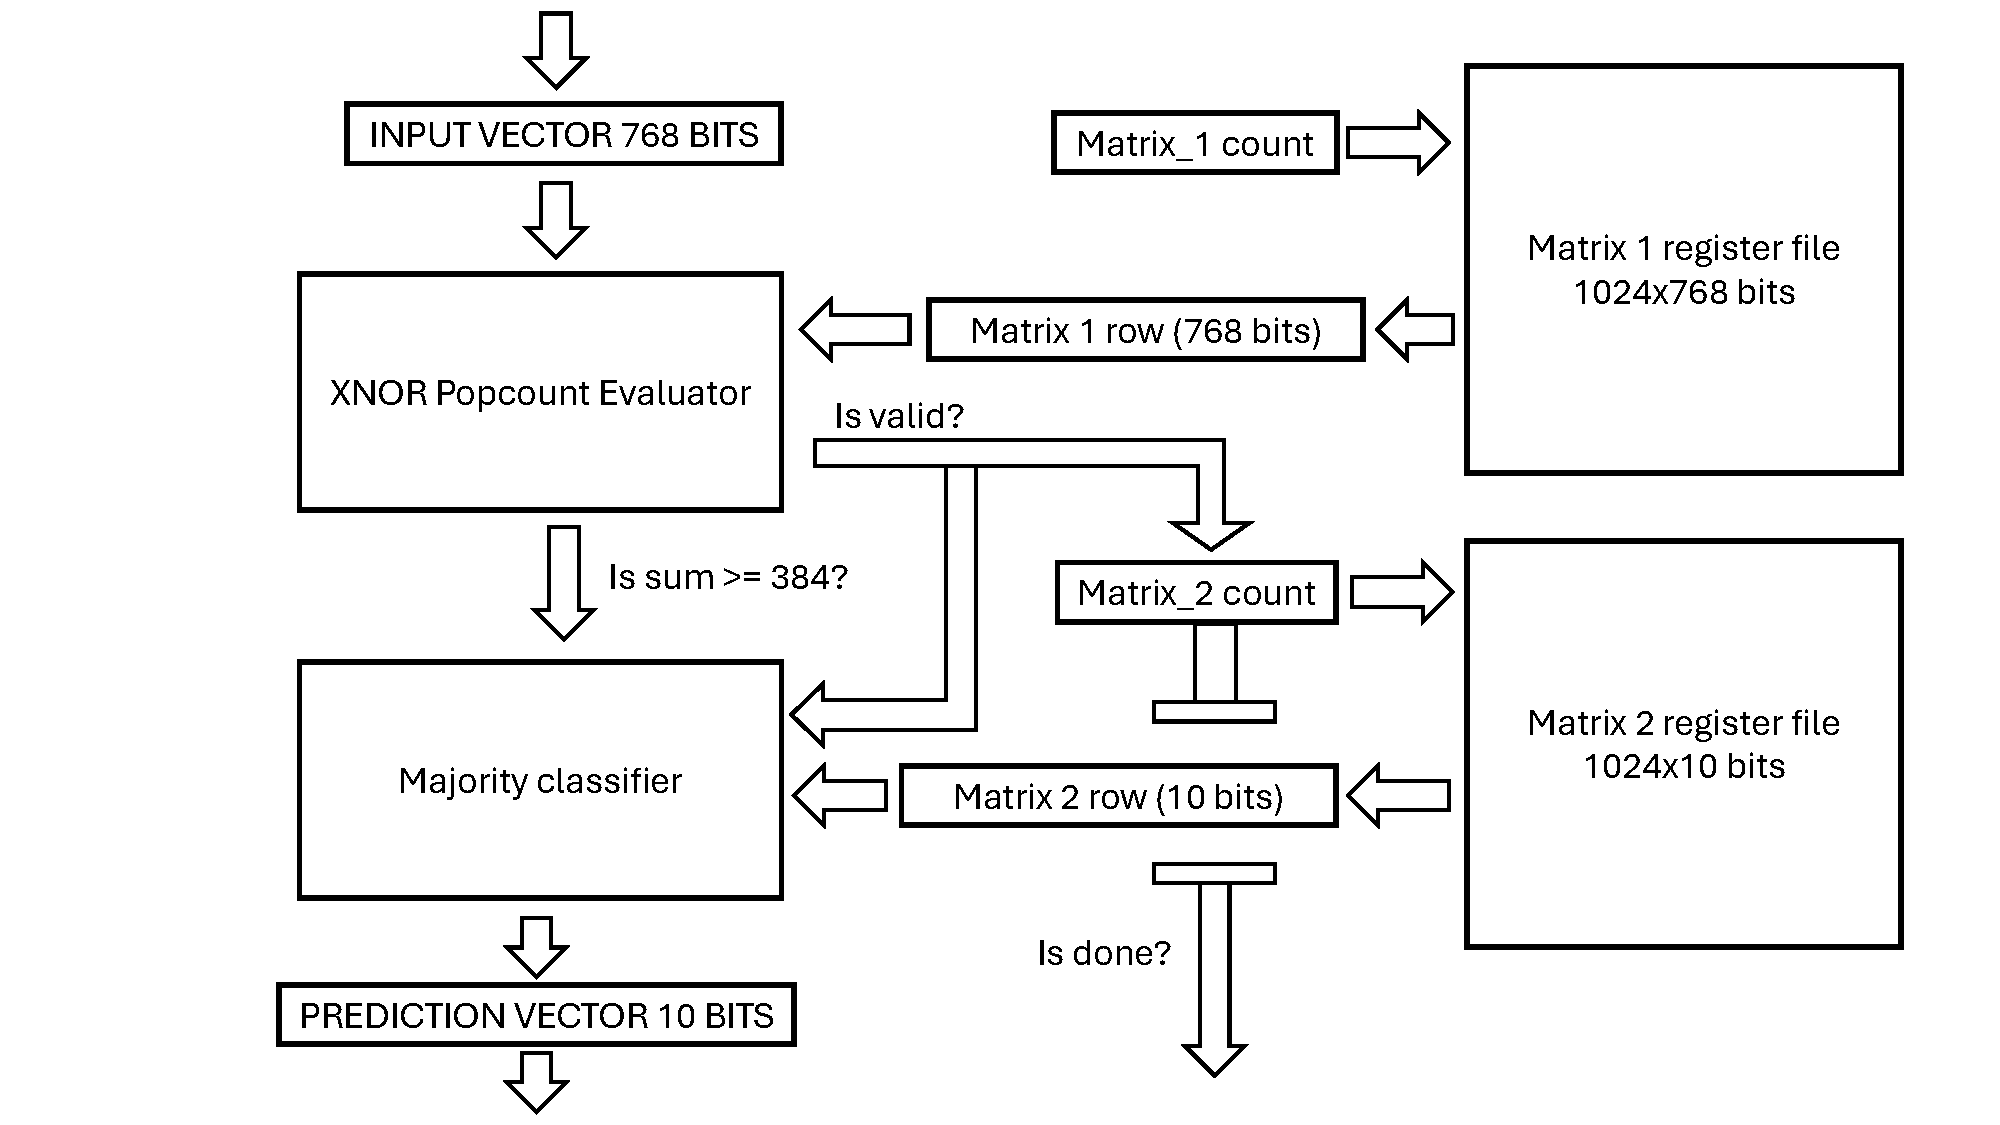
\includegraphics[width=0.4\textwidth]{overview.pdf}
    \caption{Overview of the hardware architecture.}
    \label{fig:overview}
\end{figure}

\begin{figure}[h]
    \centering
    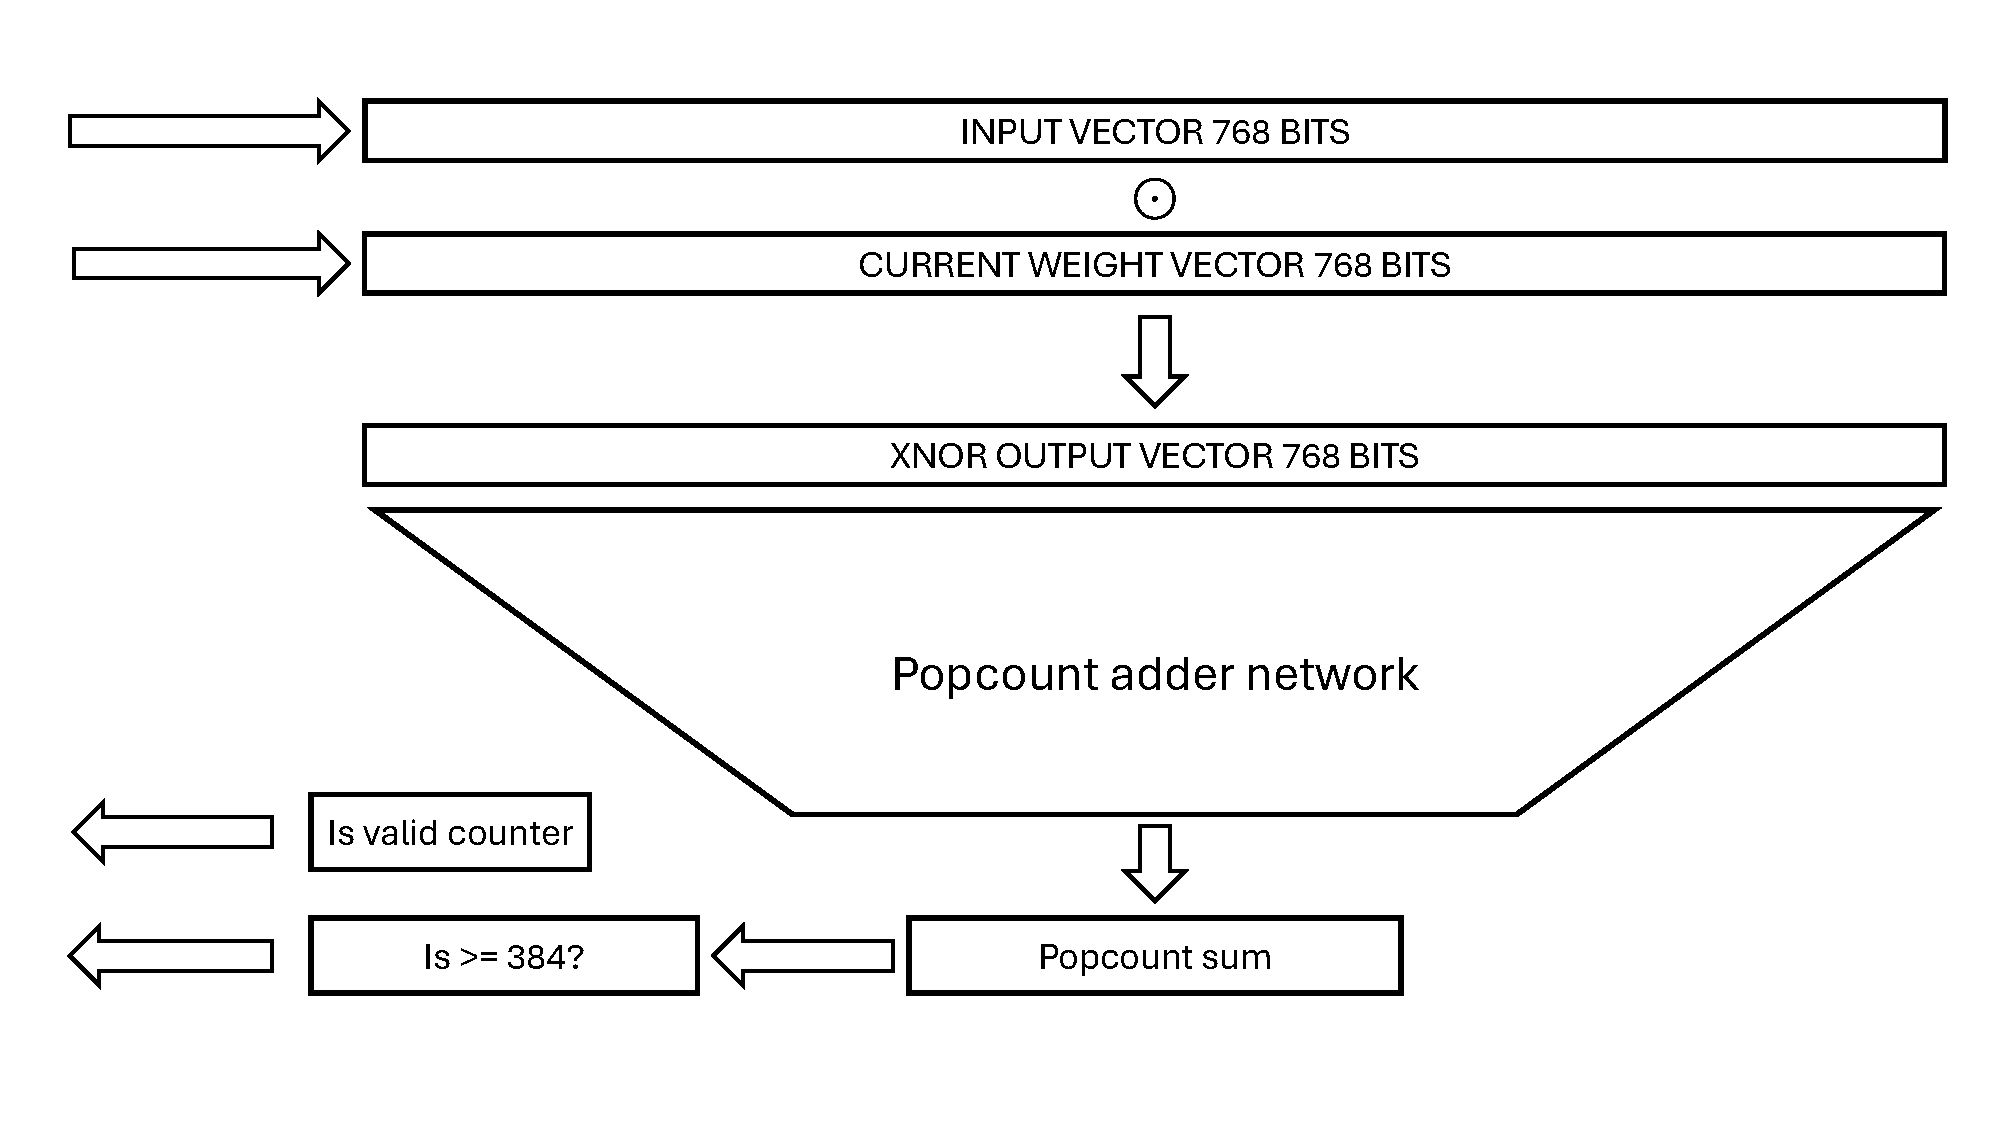
\includegraphics[width=0.4\textwidth]{Xnor_popcount.pdf}
    \caption{XNOR Popcount Evaluator.}
    \label{fig:xnor_popcount}
\end{figure}

\begin{figure}[h]
    \centering
    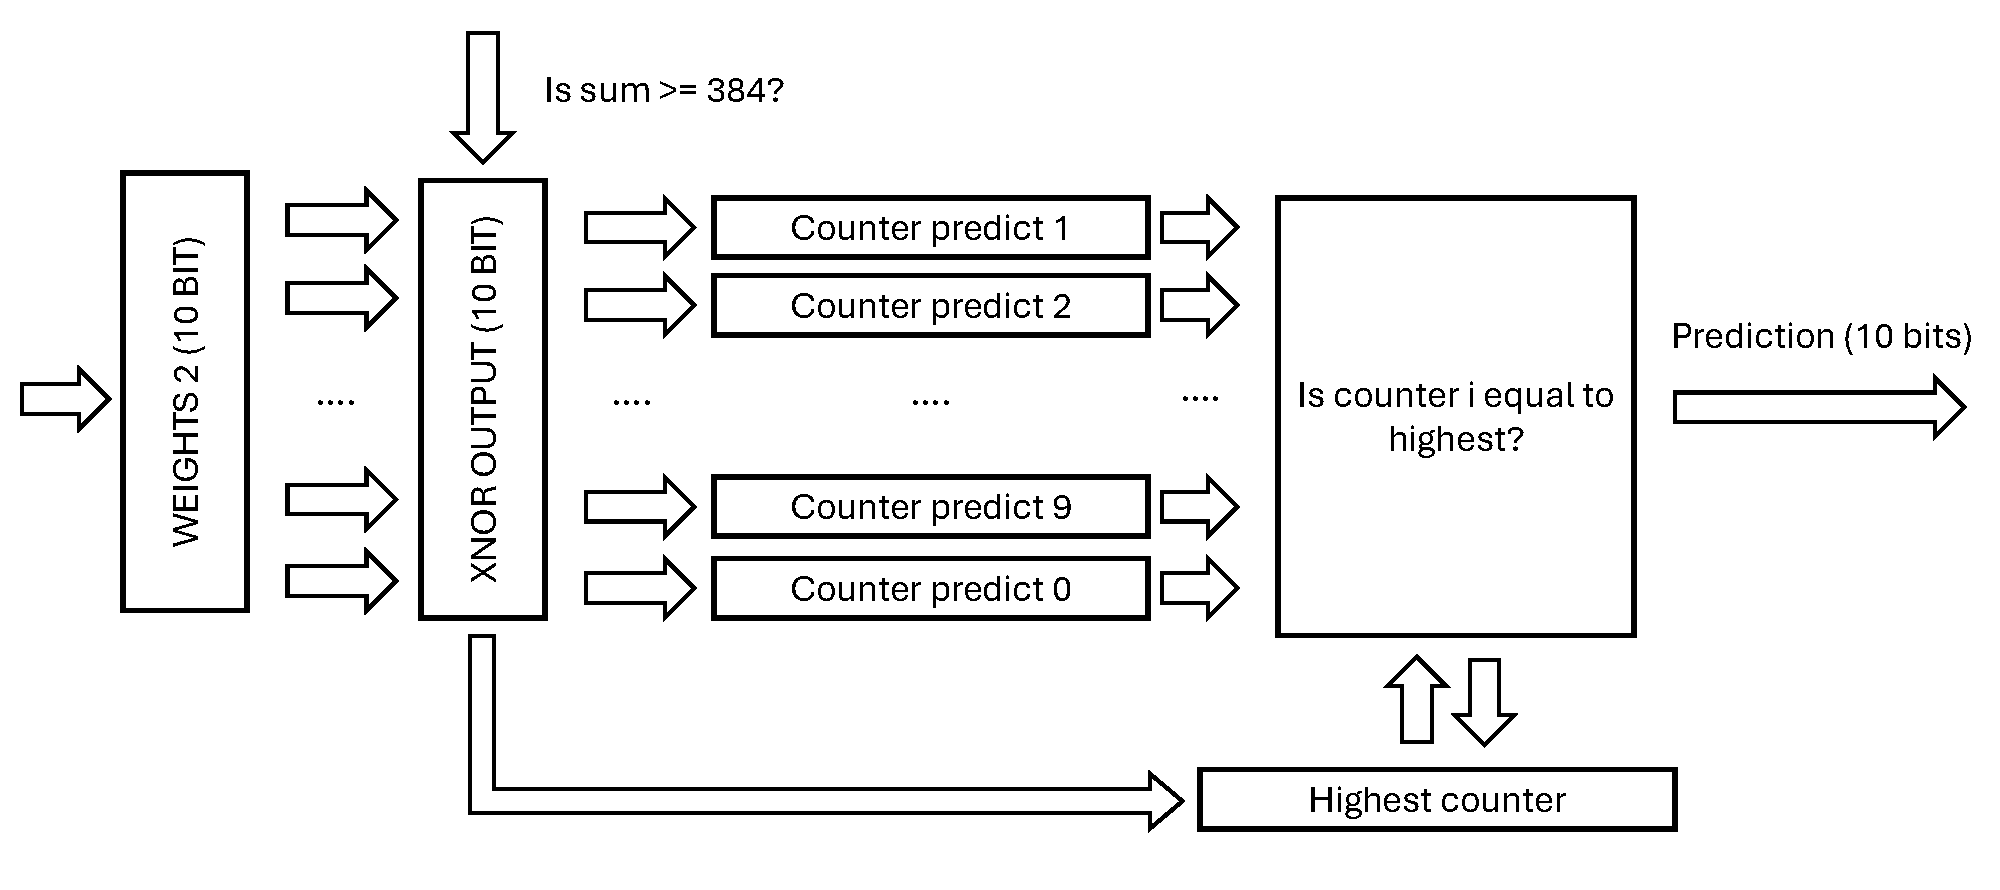
\includegraphics[width=0.4\textwidth]{majority_classifier.pdf}
    \caption{Majority Classifier.}
    \label{fig:majority_classifier}
\end{figure}



\subsection{Optimizations}
\subsubsection{Pipelining Popcount}
\label{ref:pipeline_popcount}

Instead of performing the popcount in a single clock cycle using a large Carry-Save Adder (CSA) network, our exploration in \autoref{ref:exploration_pipelining} determined that a pipelined approach with four registers between the adder stages is optimal. Thus, the popcount result becomes valid after $n=4$ cycles, with subsequent cycles producing new valid sums.

\subsubsection{LFSR-Based Majority Classifier}
\label{ref:lfsr_opt}

Initially, individual counters for each digit were used, along with a tree structure to identify the highest count. However, this structure is redundant if the highest count is tracked dynamically. Each counter is compared against the current highest count. If a counter matches the highest count and is to be incremented, the highest count is updated accordingly. This update is achieved by performing a bitwise AND operation between a 10-bit vector indicating counters equal to the highest count and a 10-bit vector indicating counters to be incremented. An OR reduction of this resultant vector determines if the highest count should increase. 
Ultimately, this approach allows the additional optimization of replacing normal counters with Linear Feedback Shift Register (LFSR) counters, which provide equivalent functionality using less area \cite{xilinx_lfsr}, as is shown in Section \ref{ref:hardware_metrics}

\subsubsection{Hidden layer size optimization}
ref to hidden size optimization 


\section{Results}
\label{sec:results}
\subsection{Simulation Setup}

The initial model, developed in PyTorch, was translated into raw NumPy operations using values of 1 and -1. Upon validation, the NumPy implementation was segmented into the XNOR Popcount and Majority Classifier components.

This segmentation allowed the generation of random test data for both components, output as text files containing 0s and 1s. These text files served as inputs for testbenches to validate the functionality of each component individually.

Additionally, text files for input vectors and corresponding labels were generated using the same method. This enabled testing the entire 10,000-image MNIST \cite{mnist} testset to verify the device's operation.

Simulations were executed using GHDL \cite{ghdl} to accelerate the simulation process and facilitate rapid testing iterations.



\subsection{Demonstration}
This section provides a detailed demonstration of the simulation results. 
\autoref{fig:waveform} presents a waveform analysis demonstrating that, after the reset signal is set low, the output vector begins displaying which counters are equal to the higest count. When the done signal is high, the output equals to the expected signal, verifying the proper operation of the designed circuit.

\begin{figure}[h]
    \centering
    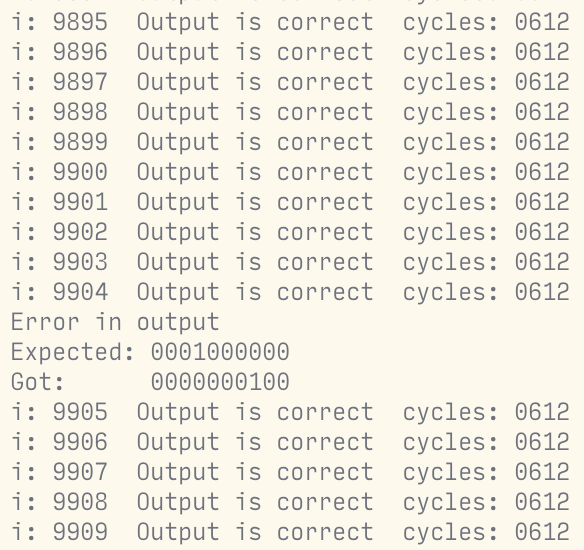
\includegraphics[width=0.2\textwidth]{./testbench.png}
    \caption{Testbench output validating the images from the MNIST test set \cite{mnist}.}
    \label{fig:testbench}
\end{figure}

\autoref{fig:testbench} displays the output of the testbench, which evaluates the entire set of 10,000 images against the full MNIST test set, confirming the functionality and accuracy of the simulation.

\begin{figure}[h]
    \centering
    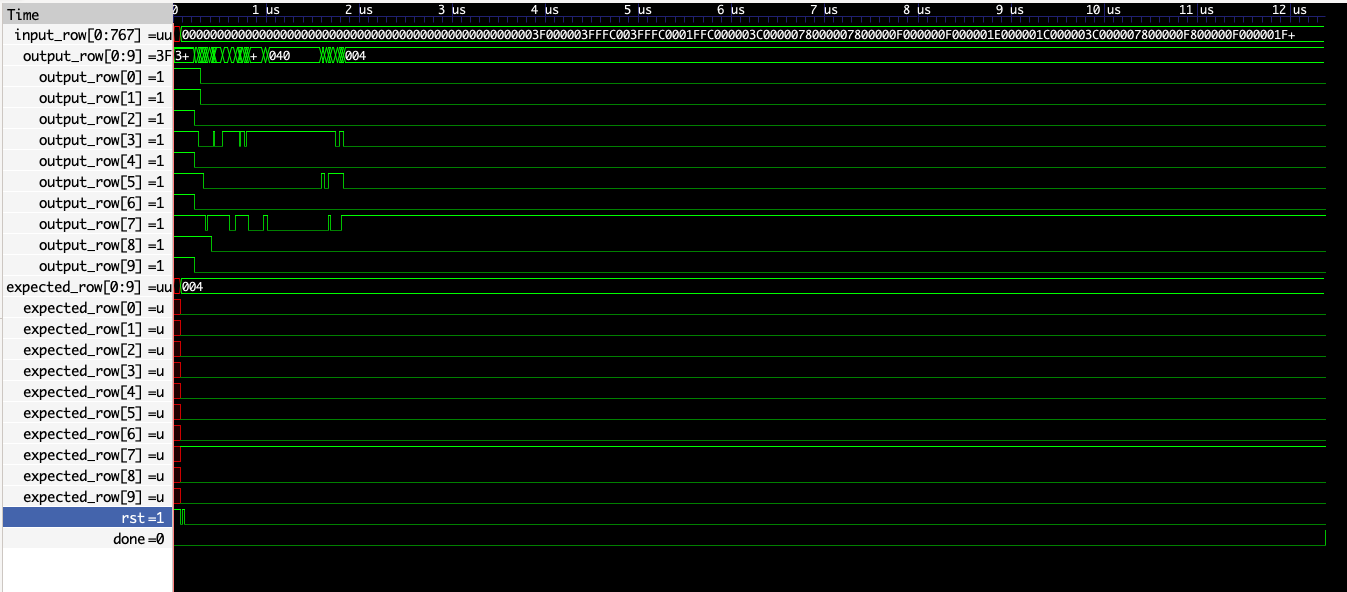
\includegraphics[width=0.4\textwidth]{./Waveform_picture.png}
    \caption{Waveform illustrating the comparison against the output\_row and expected\_row during the simulation of the testbench}
    \label{fig:waveform}
\end{figure}




% \subsection{Hardware metric results}

% This section discussed the achieved results of timing, area, power and accuracy. we present 3 optimizations: one in the hidden size, one in the popcount summing and finally one with the majority classification. Only the first optimization changes the accuracy, the rest solely affects timing, area and power. (also ref to the table saying here is table blab blab)

% // table: Run name	Popcount levels	Hidden size	Area	Power	Accuracy%	Clock period (ns)	Required clock cycles	Inference time (ns)
% original design	0	1024	113127.406	1.50E-02	95.07	2.984	1025	3059
% hidden size optimization	0	608	68376.63	1.11E-02	95.65	3.296	609	2007
% level optimization	3	608	73059.028	1.16E-02	95.65	2.842	612	1739
% lfsr optimization	3	608	70088.07	1.13E-02	95.65	2.678	612	1639



% \subsubsection{Hidden size Optimization}

% since our bnn device uses a sequential method for processing the hidden layer, the hidden size can be precisely adjusted to get the best hidden size for a given accuracy.
% Increasing the hidden size both increases the number of clock cycles:  clock cycles inference = hidden size + delay caused by xnor popcount evaluator. where hidden size >> delay cycles
% Furthermore storing the weights as is discussed in Section \ref{ref:overall_minus_rest}, is the largest contributer for area, power and timing. and the hidden size both affects the matrix 1 and 2 linearly the number of bits needed to store.

% Therefore any decrease in hidden size causes a big win in terms of performance on all metrics except accuracy.
% we first did a overview hidden size exploration to get to the 95\% target first.

% At first a global overview was done with the hidden sizes of powers of two: 64,128,256,512,1024,2048,4096
% from here it was found that 1024 was just sufficient since an accuracy of 95\% was achieved seen in \autoref{fig:line_graph_global} <- ./Global_exploration_hidden_sizes.png

% next for optimization sake every interval of 32 was tested between 512 and 1024 was tested, \autoref{fig:bar_max_achieved_accuracy <- ./Different_hidden_layer_sizes_512_1024.png} shows the max achieved accurcacy for each.

% From that it was discovered that 608 as a hidden size also reached our target of 95\% with an even greater accuracy of 95.65\%




% \subsection{Note on input size}
% \label{ref:why_768}

% Early in the design phase it was decided to use 768 instead of 784 as an input size. this was done because 768 is a much nicer number in binary and for hardware: \(768 = 512 + 256 = 2^9 + 2^8\) than 28x28=784. 
% To convert the 28*28 picture to 768 inputs, the last inputs were just dropped. in the python testing this had no impact on the accuracy. a design with 784 was never synthesized due to this early decision

\subsection{Hardware Metric Results}
\label{ref:hardware_metrics}

This section presents the results achieved in terms of timing, area, power, and accuracy. Among these, only the first optimization impacts accuracy; the latter two affect timing, area, and power metrics exclusively. A comparison of these optimizations for the total metrics is summarized in Table \ref{tab:optimization_metrics}. 

\todo{power to joules}

\begin{table}[h]
    \centering
    \caption{Comparison of Hardware Metrics Across Different Optimizations, including inference time}
    \label{tab:optimization_metrics}
    \begin{tabular}{@{}ccccccccc@{}}
        \toprule
        \textbf{Optimization} & \textbf{Area ($\mu m^2$)} & \textbf{Power (W)} & \textbf{Accuracy (\%)} & \textbf{Inference (ns)}  \\
        \midrule
        Original & 113127 & 1.50E-02 & 95.07 & 2.984 \\
        Hidden Size & 68377 & 1.11E-02 & 95.65 & 3.296 \\
        Level & 73059 & 1.16E-02 & 95.65 & 2.842 \\
        LFSR & 70088 & 1.13E-02 & 95.65 & 2.678 \\
        \bottomrule
    \end{tabular}
\end{table}

\autoref{tab:hardware_metrics} illustrates that the bulk of the area and power consumption is attributed to the weight storage in the register files. It is evident that the XNOR popcount optimization, detailed in Section \ref{ref:xnor_popcount}, results in increased area and power but enhances the timing slack. Conversely, the majority classifier optimization, as discussed in Section \ref{ref:lfsr_opt}, improves area, power, and timing slack across all metrics. Similarly, optimizing the hidden size optimizes the register files, thereby reducing timing slack, although it also incurs increases in area and power.

\begin{table}[h]
    \centering
    \caption{Hardware Metrics for Device Parts: Impact of Optimizations}
    \label{tab:hardware_metrics}
    \begin{tabular}{@{}lcccc@{}}
        \toprule
        \textbf{Device Part} & \textbf{Area (\(\mu m^2\))} & \textbf{Power (W)} & \textbf{Time Slack (ps)} \\
        \midrule
        Register Files Old & 104334 & 1.36E-02 & 7016 \\
        Register Files New & 62653 & 1.00E-02 & 6704 \\
        XNOR Popcount Old & 4487 & 7.30E-04 & 7957 \\
        XNOR Popcount New & 6095 & 1.08E-03 & 8973 \\
        Majority Classifier Old & 4307 & 6.86E-04 & 8825 \\
        Majority Classifier New & 1340 & 2.38E-04 & 9046 \\
        \bottomrule
    \end{tabular}
\end{table}

\subsubsection{Note on Input Size}
\hfill\\
\label{ref:why_768}

During the design phase, the input size was set to 768 instead of 784 to align with hardware efficiency, as 768 (\(2^9 + 2^8\)) simplifies binary implementation. The 28x28 input image was truncated to 768 inputs by excluding the last 16 pixels. Empirical testing confirmed no accuracy impact, hence, 784-input designs were not pursued.


\subsection{Hidden Size Optimization}

Given that our Binary Neural Network (BNN) device employs a sequential approach for processing the hidden layer, it is crucial to finely tune the hidden size to balance accuracy and hardware efficiency. Increasing the hidden size directly correlates with an increase in the number of clock cycles required for inference.
Since the hidden size affects both the first and second weight register files proportionally, any reduction in hidden size guarantees substantial gains across all hardware metrics except accuracy.

An initial broad exploration was conducted using hidden sizes that are powers of two: 64, 128, 256, 512, 1024, 2048, 4096. From this analysis, it was determined that a hidden size of 1024 was sufficient to achieve the target accuracy of 95\%, as illustrated in \autoref{fig:line_graph_global}.

\begin{figure}[h]
    \centering
    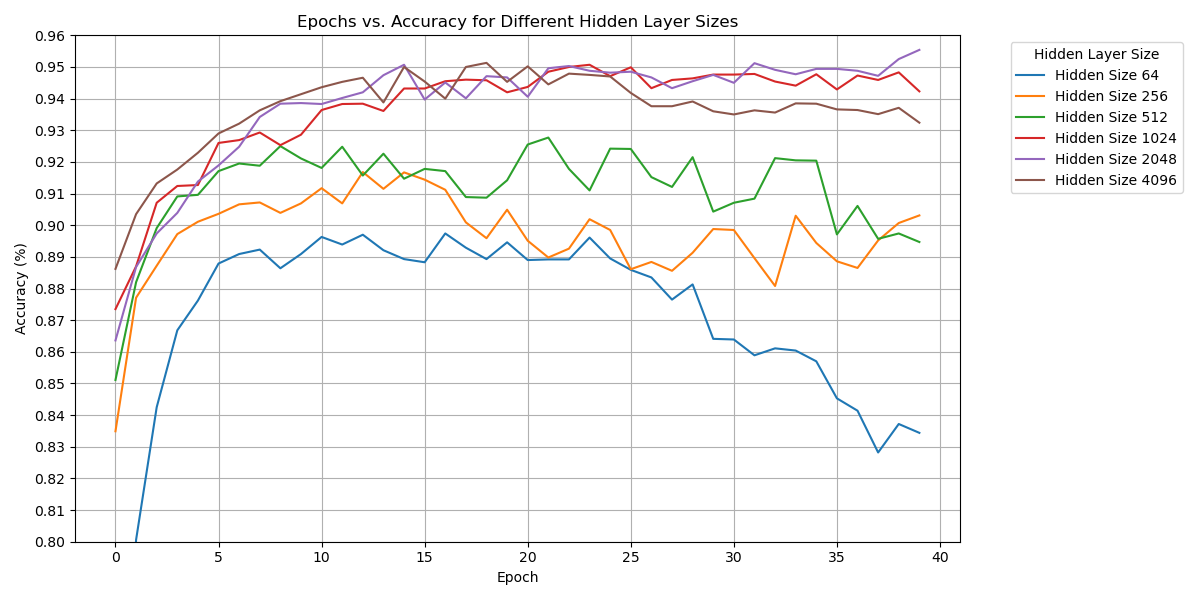
\includegraphics[width=0.4\textwidth]{Global_exploration_hidden_sizes.png}
    \caption{Global exploration of hidden sizes and their impact on accuracy.}
    \label{fig:line_graph_global}
\end{figure}

For further optimization, the hidden size was refined in increments of 32 between 512 and 1024. The maximum achieved accuracy for each hidden size within this range is depicted in \autoref{fig:bar_max_achieved_accuracy}. Through this fine-grained exploration, a hidden size of 608 was identified as optimal, reaching the target accuracy of 95\% with a slight improvement to 95.65\%.

\begin{figure}[h]
    \centering
    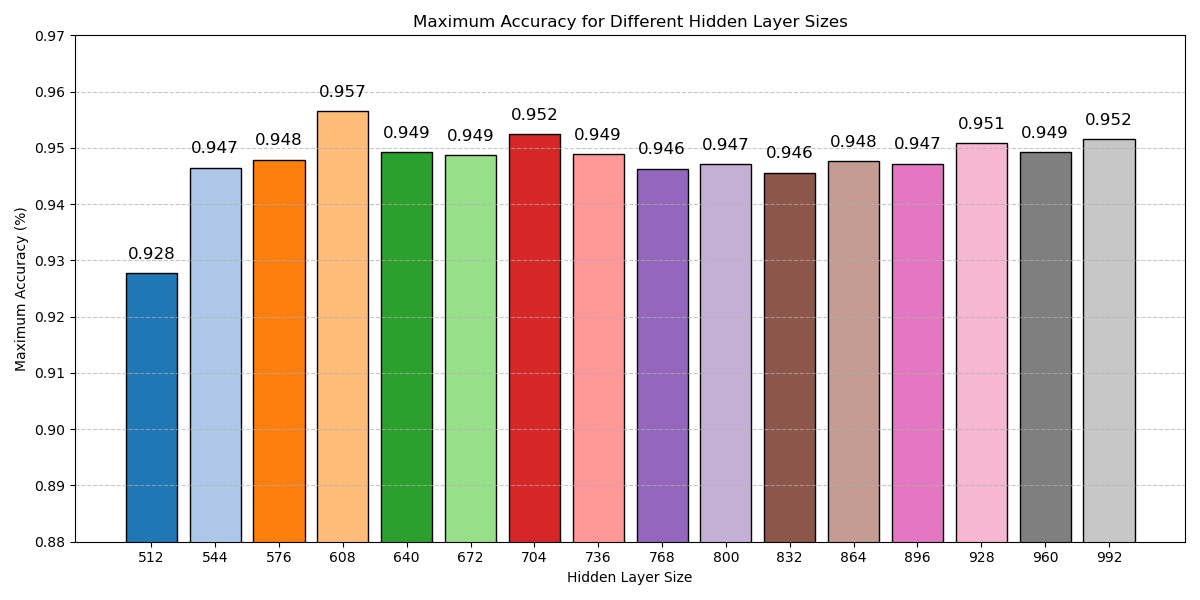
\includegraphics[width=0.4\textwidth]{Different_hidden_layer_sizes_512_1024.png}
    \caption{Maximum achieved accuracy for different hidden layer sizes between 512 and 1024.}
    \label{fig:bar_max_achieved_accuracy}
\end{figure}

\subsection{XNOR popcount Optimization}
\label{ref:xnor_popcount}

This section explores optimizing the XNOR popcount module with a focus on reducing timing slack to enhance clock speed. Given that the majority of area and power consumption arises from the register files, as indicated in \ref{ref:hardware_metrics}, the strategy centered on minimizing slack to improve performance efficiency.

\subsubsection{Initial Approach: Direct CSA Tree Implementation}
\hfill\\

The initial exploration of the XNOR popcount involved synthesizing a direct Carry-Save Adder (CSA) tree to provide a foundational understanding of the basic performance metrics. This method utilizes a full direct CSA tree to compute the population count. Only the XNOR popcount part was synthesized, which facilitated a more rapid assessment. The results for this direct CSA implementation, including area, timing, and power, are summarized in Table \ref{tab:direct_csa}. This direct implementation serves as a reference point before introducing pipelining for performance improvements.


\begin{table}[h]
    \centering
    \caption{Metrics for Direct CSA Tree Implementation}
    \label{tab:direct_csa}
    \begin{tabular}{@{}ccc@{}}
        \toprule
        \textbf{Area ($\mu m^2$)} & \textbf{Timing (ps)} & \textbf{Power (W)} \\
        \midrule
          4487 & 7957 & 7.30E-04 \\
        \bottomrule
    \end{tabular}
\end{table}


\subsubsection{First-Level Pipelining Exploration}
\hfill\\

To optimize performance and reduce the required minimum slack, pipelining stages were introduced within the CSA network. This exploration started by examining a single intermediary level of sum registers. These registers accumulate counts up to a specified maximum before passing their sum to the next stage. For example, a configuration with a maximum sum of 64 means that the CSA tree computes partial sums of the XNOR output vector in chunks of 64, leading to intermediate registers each counting up to 64. These intermediate sums are then aggregated by another CSA tree to produce the final output sum. Various configurations were explored, where the maximum sums ranged from 16 to 384. Table \ref{tab:first_level} presents the area, timing, and power metrics for these configurations.


\begin{table}[h]
    \centering
    \caption{Metrics for CSA Tree with One Level of Pipelining}
    \label{tab:first_level}
    \begin{tabular}{@{}ccccc@{}}
        \toprule
        \textbf{Max Sum} & \textbf{Area ($\mu m^2$)} & \textbf{Timing (ps)} & \textbf{Power (W)} \\
        \midrule
        16 & 6664.63 & 8318 & 1.30E-03 \\
        32 & 5739.482 & 8458 & 1.06E-03 \\
        48 & 5298.986 & 8604 & 9.40E-04 \\
        64 & 5241.796 & 8618 & 9.58E-04 \\
        96 & 4986.702 & 8528 & 8.79E-04 \\
        128 & 4937.758 & 8457 & 8.47E-04 \\
        192 & 4793.054 & 8251 & 8.41E-04 \\
        256 & NA & NA & NA \\
        384 & NA & NA & NA \\
        \bottomrule
    \end{tabular}
\end{table}

\subsubsection{Two-Level Pipelining Exploration}
\hfill\\

To further refine the pipelining strategy, a two-level configuration was tested. Due to the extensive nature of possible combinations, a targeted exploration approach was used. This began with the insertion of an additional level of sum registers, capable of holding up to 256 counts, between the initial sum of 64 and the final output sum from the best performing configuration in Table \ref{tab:first_level}. Each test subsequently modified the maximum sum at the stage exhibiting the worst timing in the previous test. For example, in the configuration where Level 1 had a maximum sum of 64 and Level 2 had 256, the worst timing was observed between the input and the 64-bit stage. This led to the next test where the Level 1 sum was reduced to 16. The configurations explored and their results are detailed in Table \ref{tab:two_level}. This iterative approach aimed to minimize the worst timing while considering area and power metrics.


\begin{table}[h]
    \centering
    \caption{Metrics for CSA Tree with Two Levels of Pipelining}
    \label{tab:two_level}
    \begin{tabular}{@{}cccccc@{}}
        \toprule
        \textbf{Levels} & \textbf{Area ($\mu m^2$)} & \textbf{Timing (ps)} & \textbf{Power (W)} & \textbf{Worst} \\
        \midrule
        64, 256 & 5365 & 8617 & 1.01E-03 & input $\rightarrow$ 64 \\
        16, 256 & 6865 & 8740 & 1.36E-03 & 16 $\rightarrow$ 256 \\
        48, 192 & 5526 & 8750 & 9.84E-04 & input $\rightarrow$ 48 \\
        32, 192 & 5960 & 8834 & 1.11E-03 & input $\rightarrow$ 32 \\
        24, 192 & 5999 & 8851 & 1.07E-03 & 192 $\rightarrow$ out\\
        24, 384 & 5900 & 8740 & 1.05E-03 & 24 $\rightarrow$ 384 \\
        \bottomrule
    \end{tabular}
\end{table}

\subsubsection{Three-Level Pipelining Exploration}
\hfill\\

Finally, a three-level pipelining configuration was investigated to achieve further optimization. Starting with the best-performing two-level configuration (24 for Level 1 and 192 for Level 2), a third level was added with the maximum sum set to 384. The rationale was to mitigate the worst timing observed at the 192 to output transition by adding another intermediary stage. Subsequent configurations tested included 24, 192, 384, and 16, 128, 384 to observe the effects on area and timing. The configuration of 24 for Level 1, 192 for Level 2, and 384 for Level 3 demonstrated the best balance across area, timing, and power, making it the chosen configuration. 

Introducing an additional layer does not yield better timing performance, as the critical timing slack occurs between the 384 sum level and the output. Given that 768 cannot be divided into larger segments than 384, further division does not mitigate this bottleneck. 
The results for the three-level pipelining exploration are provided in Table \ref{tab:three_level}.

\begin{table}[h]
    \centering
    \caption{Metrics for CSA Tree with Three Levels of Pipelining}
    \label{tab:three_level}
    \begin{tabular}{@{}ccccccc@{}}
        \toprule
        \textbf{Levels} & \textbf{Area ($\mu m^2$)} & \textbf{Timing (ps)} & \textbf{Power (W)} & \textbf{Worst} \\
        \midrule
        24, 192, 384 & 6095 & 8973 & 1.08E-03 & 384 $\rightarrow$ out\\
        16, 192, 384 & NA & NA & NA & NA \\
        16, 128, 384 & 7108 & 8979 & 1.40E-03 & 16 $\rightarrow$ 128 \\
        \bottomrule
    \end{tabular}
\end{table}

\subsubsection{Conclusion XNOR Popcount exploration}
\hfill\\

Through methodical exploration of various pipelining levels, the implementation of intermediary sum registers proved effective in enhancing the XNOR popcount performance. The three-level configuration with maximum sums of 24, 192, and 384 provided the most optimal trade-off between area, timing, and power, as indicated by the iterative testing and metrics obtained.





\section{Discussion}
\label{sec:discussion}
\todo{timing is slower in lower hidden size}

%   - [ ] accuracy differences were not that great and partially due to random chance
	% - [ ] Hyperparameter tuning might be overfitting on the testset
    \subsection{Accuracy Differences and Hyperparameter Tuning}
    The observed differences in accuracy were not substantial and might be attributed to random variations rather than significant improvements or degradations in performance. Additionally, there is a possibility that hyperparameter tuning may have led to overfitting on the test set. This means that while the model performs well on the specific test data, it may not generalize as effectively to new, unseen data.
    % - [ ] Rationale
    \subsection{Rationale for Design Decisions}
    %   - [ ] somewhere needs to be put a better reasoning why 2 matrices are more efficient: either have 1024 counters = excessive or 1024x768 counts which is slow and area gains are low
    \begin{itemize}
        \item Efficiency of Two Matrices
        Using two matrices is more efficient for several reasons. Employing 1024 counters is considered excessive in terms of hardware resources. Additionally, utilizing 1024x768 counts can be slow and offers minimal area gains, making it an inefficient choice.
         % 	- [ ] why not CNN decision: would probably require somewhere a linear layer anyways, or a large number of layers vastly reducing speed
        \item Decision Against Using CNN
        Implementing a CNN would likely require a linear layer at some stage or a substantial number of layers, which would significantly reduce speed. The potential complexity and depth of CNNs would lead to a decrease in operational speed, making them less suitable for the intended application.
         % 	- [ ] Small section that weight memory is most of the area
        \item Impact of Weight Memory
        Weight memory constitutes a significant portion of the total area. Managing and optimizing weight memory is crucial to maintaining an efficient design.
    \end{itemize}
	%     - [ ] section on hardware possible strategies given Fully connected bnn
    \subsection{Hardware Possible Strategies for Fully Connected BNN}
    \begin{itemize}
        % 	    - [ ] subsubsection strategy do everything sequentially
        \item Sequential Strategy
        Performing all operations sequentially is a simpler approach but might be unnecessarily slow. It offers minimal area and power savings due to the mandatory weight storage requirements.
        % 	    - [ ] subsubsection strategy do everything in parallel in one tick
        \item Parallel Strategy
        Executing all operations in parallel within a single clock tick can be extremely fast. However, this method requires a large amount of hardware resources, making it impractical for many applications due to its substantial area and power demands.
        % 	    - [ ] subsubsection strategy mixed approach, since parallel would be huge and sequentially would be unneccesary slow for little area and power gains due to weights storage that is mandatory
        \item Mixed Strategy
        The hybrid approach to processing combines elements of both sequential and parallel processing strategies. By blending these methods, it seeks to leverage the strengths of each while mitigating their respective drawbacks. This approach aims to strike a balance between speed and resource usage, optimizing performance without excessively draining area and power. It aims to avoid the inefficiencies inherent in purely sequential processing, such as long execution times, while also sidestepping the challenges of purely parallel processing, such as increased complexity and potential bottlenecks. Ultimately, the hybrid approach offers a compromise solution that aims to deliver efficient and effective processing capabilities across various applications and domains.
    \end{itemize}
\section{Conclusions}
\label{sec:conclusions}
	- [ ] exploration of multiple hidden sizes was very benificial
	- [ ] overall bottleneck mostly from memory
	- [ ] optimization caused 2x performance increase and 38\% reduction in size and XXX\% reduction of joules per inference


\todo{future work}
	- [done ] subsection better memory library
	- [done ] subsection also try 729 as input size for xnor popcount csa network

\section{future work}
\label{sec:future}
	\subsection{Better Memory Library}
Improving the memory library is an important step for future implementations of the BNN. In this paper, the memory components in our design are based on standard libraries, which may not be optimized for the specific needs of BNN operations. By developing or integrating a specialized memory library specifically for binary operations, we can significantly reduce the access time and energy consumption. This specialized memory can include optimized SRAM or emerging memory technologies like ReRAM, which are more suited for the frequent read-write cycles in BNN computations. A better memory library will contribute to lower latency and higher efficiency, ultimately improving the overall performance of the BNN hardware.

	\subsection{Input Size Optimization with 729}
Another promising area for future work is experimenting with an input size of 729 for the XNOR-popcount CSA network. This might enhance the alignment and efficiency of the XNOR and popcount operations. This approach could lead to more balanced computational loads and possibly reduce the overall hardware complexity. Testing this input size may uncover further optimizations in terms of area and power without compromising accuracy.

\printbibliography

\newpage


\appendix
\label{appendix}

\section{Mathematical Foundations for Hardware Implementations}

\label{appendix:bnn_maths}

\subsection{First matrix multiplication with activation}

This section demonstrates that performing matrix-vector multiplication followed by a hard activation is equivalent to using XNOR operations, popcount, and a subsequent comparison.
The matrix-vector multiplication \(\mathbf{A} \mathbf{b}\) shown in Equation \ref{eq:matrix_vector_multiplication} results in a vector \(\mathbf{c}\). Each element \(c_i\) of this vector is obtained by the dot product of the \(i\)-th row of matrix \(\mathbf{A}\) with vector \(\mathbf{b}\), as described in Equation \ref{eq:dot_product}. This can be further expanded into component-wise multiplication and summation (Equation \ref{eq:component_wise_dot}). When elements \(a_{ij}\) and \(b_j\) are binary (\(1\) or \(-1\)), we map them to \(1\) and \(0\) respectively, as shown in Equation \ref{eq:mapping}, enabling the use of XNOR for the multiplication, as described in Equation \ref{eq:xnor}.

\begin{figure}[ht]
    \centering
    \begin{equation}
    \mathbf{c} = \mathbf{A} \mathbf{b}
    \label{eq:matrix_vector_multiplication}
    \end{equation}

    \begin{equation}
    c_i = \sum_{j=1}^n a_{ij} b_j
    \label{eq:dot_product}
    \end{equation}

    \begin{equation}
    c_i = \sum_{j=1}^n (a_{ij} \cdot b_j)
    \label{eq:component_wise_dot}
    \end{equation}

    \begin{equation}
    a'_{ij} = \begin{cases}
    1 & \text{if } a_{ij} = 1 \\
    0 & \text{if } a_{ij} = -1
    \end{cases}, \quad
    b'_j = \begin{cases}
    1 & \text{if } b_j = 1 \\
    0 & \text{if } b_j = -1
    \end{cases}
    \label{eq:mapping}
    \end{equation}

    \begin{equation}
    a_{ij} \cdot b_j = \text{XNOR}(a'_{ij}, b'_j)
    \label{eq:xnor}
    \end{equation}

    \caption{Matrix-vector multiplication and equivalent dot product representation.}
    \label{fig:matrix_vector_multiplication}
\end{figure}


\begin{figure}[ht]
    \centering
    \begin{equation}
    c = \sum_{i=1}^n a_i b_i
    \label{eq:dot_product_sum}
    \end{equation}

    \begin{equation}
    c = \left|\{c_i \mid c_i = 1\}\right| - \left|\{c_i \mid c_i = -1\}\right|
    \label{eq:dot_product_count}
    \end{equation}

    \begin{equation}
    |\{c_i \mid c_i = -1\}| = n - |\{c_i \mid c_i = 1\}|
    \label{eq:negative_count}
    \end{equation}

    \begin{equation}
    a \cdot b = 2 \left|\{c_i \mid c_i = 1\}\right| - n
    \label{eq:dot_product_simplified}
    \end{equation}

    \begin{equation}
    \text{activation}(c) = \begin{cases}
    1 & \text{if } 2 \left|\{c_i \mid c_i = 1\}\right| \geq n \\
    -1 & \text{otherwise}
    \end{cases}
    \label{eq:activation_function}
    \end{equation}

    \begin{equation}
    \text{activation}(c) = \begin{cases}
    1 & \text{if } \left|\{c_i \mid c_i = 1\}\right| \geq \frac{n}{2} \\
    -1 & \text{otherwise}
    \end{cases}
    \label{eq:activation_function_half}
    \end{equation}

    \begin{equation}
    \text{activation}(a \text{ XNOR } b) = \begin{cases}
    1 & \text{if } \text{popcount}(a \text{ XNOR } b) \geq \frac{n}{2} \\
    -1 & \text{otherwise}
    \end{cases}
    \label{eq:activation_xnor}
    \end{equation}

    \caption{Dot product calculation and activation function.}
    \label{fig:dot_product_activation}
\end{figure}

In Figure \ref{fig:dot_product_activation}, Equation \ref{eq:dot_product_sum} sums the products of the components. Equation \ref{eq:dot_product_count} translates the sum into a count of \(1\)s and \(-1\)s. The total count of \(-1\)s can be expressed as the complement of the count of \(1\)s (Equation \ref{eq:negative_count}). The dot product simplifies to Equation \ref{eq:dot_product_simplified}. The activation function (Equation \ref{eq:activation_function}) sets the output based on the threshold condition, which can also be expressed equivalently as shown in Equation \ref{eq:activation_function_half}. This is related to the XNOR operation in Equation \ref{eq:activation_xnor}, where the activation depends on the population count of the XNOR operation being greater than or equal to half the length of the vector.


\subsection{maths second matrix}
\todo{subsubsection maths is same but now the actual highest popcount needs to be found}




\vspace{12pt}
\showtodocount


\end{document}


